\documentclass[11pt]{article}
\usepackage[a4paper,margin=1in]{geometry}
\usepackage{amsmath,amssymb,amsthm}
\usepackage{tikz}
\usepackage{booktabs}
\usepackage[hidelinks]{hyperref}
\hypersetup{pdftitle={Nine rectangles of equal perimeter in a square},pdfauthor={Vamshi Jandhyala}}
\setlength{\parskip}{0.4em}
\setlength{\parindent}{0pt}

\newtheorem{theorem}{Theorem}
\newtheorem{lemma}{Lemma}

\title{Nine rectangles of equal perimeter, no two alike, in a square}
\author{Vamshi Jandhyala}
\date{}


\begin{document}
\maketitle
\vspace{-2em}

\begin{abstract}
A square can be cut into nine rectangles that all have the same perimeter and no two of which are congruent, for instance an $84\times84$ square into pieces of perimeter $130$. Nine is the least number of pieces for which this is possible, and up to rotation, reflection and scaling there are exactly five such dissections with nine pieces. The proof is an exact enumeration over all combinatorial types of dissection, carried out by two independent programs.
\end{abstract}

\section{The question}

Cut a square into rectangles so that every piece has the same perimeter. Cutting it into $n$ equal strips does this, and so does any grid of equal squares. The question is whether it can be done with pieces that are all different. The question was asked on the newsgroup \texttt{alt.math.recreational} in 2006~\cite{vanvera}, raised again by Nandakumar~\cite[p.~5]{nandakumar}, who guessed that no such square exists, and asked on MathOverflow in 2018~\cite{mo}. It is a cousin of the equal-area problem, where the least number of pairwise non-congruent rectangles of equal area into which a square can be cut is seven~\cite{dalfo}.

For equal perimeters the answer is yes. Figure~\ref{fig:84} shows an $84\times 84$ square cut into nine rectangles, each with perimeter $130$, that is, each with width plus height equal to $65$. Their dimensions, in order of area, are
\[
59\times6,\quad 10\times55,\quad 53\times12,\quad 15\times50,\quad 48\times17,\quad 21\times44,\quad 43\times22,\quad 38\times27,\quad 31\times34
\]
with areas $354, 550, 636, 750, 816, 924, 946, 1026, 1054$%, which add up to $84^2=7056$. Two rectangles with the same perimeter are congruent exactly when they have the same area, since width and height are then the roots of the same quadratic. So ``no two congruent'' can be checked by looking at the areas, and Nandakumar's phrasing (equal perimeters, different areas) asks for the same thing.

\begin{figure}[ht]
\centering
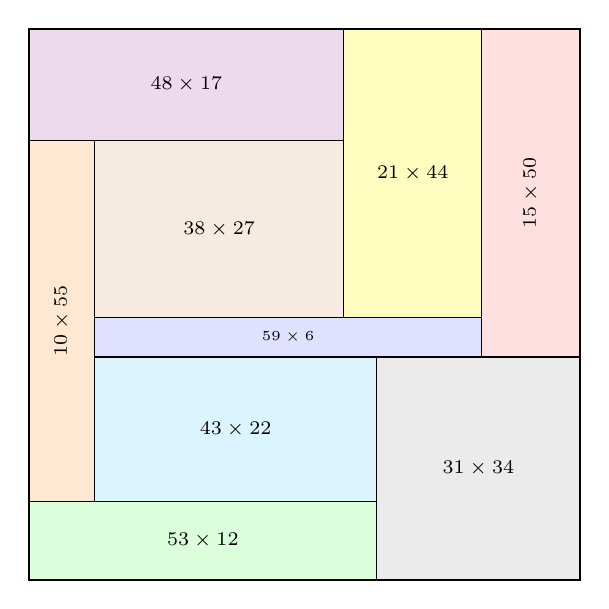
\begin{tikzpicture}[x=0.08333cm,y=0.08333cm]
\filldraw[fill=blue!12,draw=black,line width=0.4pt] (10,34) rectangle (69,40);
\node[font=\tiny] at (39.5,37.0) {$59\times6$};
\filldraw[fill=orange!18,draw=black,line width=0.4pt] (0,12) rectangle (10,67);
\node[font=\scriptsize,rotate=90] at (5.0,39.5) {$10\times55$};
\filldraw[fill=green!14,draw=black,line width=0.4pt] (0,0) rectangle (53,12);
\node[font=\scriptsize] at (26.5,6.0) {$53\times12$};
\filldraw[fill=red!12,draw=black,line width=0.4pt] (69,34) rectangle (84,84);
\node[font=\scriptsize,rotate=90] at (76.5,59.0) {$15\times50$};
\filldraw[fill=violet!14,draw=black,line width=0.4pt] (0,67) rectangle (48,84);
\node[font=\scriptsize] at (24.0,75.5) {$48\times17$};
\filldraw[fill=yellow!25,draw=black,line width=0.4pt] (48,40) rectangle (69,84);
\node[font=\scriptsize] at (58.5,62.0) {$21\times44$};
\filldraw[fill=cyan!14,draw=black,line width=0.4pt] (10,12) rectangle (53,34);
\node[font=\scriptsize] at (31.5,23.0) {$43\times22$};
\filldraw[fill=brown!16,draw=black,line width=0.4pt] (10,40) rectangle (48,67);
\node[font=\scriptsize] at (29.0,53.5) {$38\times27$};
\filldraw[fill=gray!16,draw=black,line width=0.4pt] (53,0) rectangle (84,34);
\node[font=\scriptsize] at (68.5,17.0) {$31\times34$};
\draw[line width=0.9pt] (0,0) rectangle (84,84);
\end{tikzpicture}

\caption{An $84\times84$ square cut into nine pairwise non-congruent rectangles, each of perimeter $130$.}
\label{fig:84}
\end{figure}

Once one example exists, the natural questions are how few pieces suffice and how many dissections there are. Call two dissections equivalent if one is carried to the other by a rotation, a reflection or a change of scale.

\begin{theorem}\label{thm:main}
For $2\le n\le 8$ no square can be cut into $n$ pairwise non-congruent rectangles of equal perimeter. For $n=9$ there are exactly five such dissections up to equivalence. Scaled to integer coordinates in lowest terms, they live in squares of side $72$, $84$, $86$, $161$ and $165$, with common perimeters $130$, $130$, $130$, $260$ and $260$ (Figure~\ref{fig:all5} and Table~\ref{tab:all5}).
\end{theorem}

\begin{figure}[ht]
\centering
\begin{minipage}[b]{0.19\textwidth}\centering
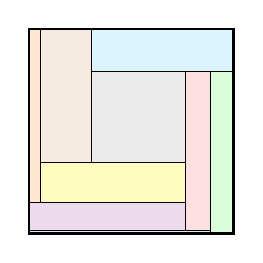
\begin{tikzpicture}[x=0.03611cm,y=0.03611cm]
\filldraw[fill=blue!12,draw=black,line width=0.4pt] (0,0) rectangle (64,1);
\filldraw[fill=orange!18,draw=black,line width=0.4pt] (0,11) rectangle (4,72);
\filldraw[fill=green!14,draw=black,line width=0.4pt] (64,0) rectangle (72,57);
\filldraw[fill=red!12,draw=black,line width=0.4pt] (55,1) rectangle (64,57);
\filldraw[fill=violet!14,draw=black,line width=0.4pt] (0,1) rectangle (55,11);
\filldraw[fill=yellow!25,draw=black,line width=0.4pt] (4,11) rectangle (55,25);
\filldraw[fill=cyan!14,draw=black,line width=0.4pt] (22,57) rectangle (72,72);
\filldraw[fill=brown!16,draw=black,line width=0.4pt] (4,25) rectangle (22,72);
\filldraw[fill=gray!16,draw=black,line width=0.4pt] (22,25) rectangle (55,57);
\draw[line width=0.9pt] (0,0) rectangle (72,72);
\end{tikzpicture}\\[2pt]{\footnotesize side 72, perimeter 130}
\end{minipage}\hfill
\begin{minipage}[b]{0.19\textwidth}\centering
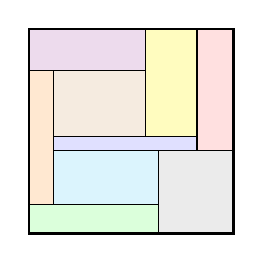
\begin{tikzpicture}[x=0.03095cm,y=0.03095cm]
\filldraw[fill=blue!12,draw=black,line width=0.4pt] (10,34) rectangle (69,40);
\filldraw[fill=orange!18,draw=black,line width=0.4pt] (0,12) rectangle (10,67);
\filldraw[fill=green!14,draw=black,line width=0.4pt] (0,0) rectangle (53,12);
\filldraw[fill=red!12,draw=black,line width=0.4pt] (69,34) rectangle (84,84);
\filldraw[fill=violet!14,draw=black,line width=0.4pt] (0,67) rectangle (48,84);
\filldraw[fill=yellow!25,draw=black,line width=0.4pt] (48,40) rectangle (69,84);
\filldraw[fill=cyan!14,draw=black,line width=0.4pt] (10,12) rectangle (53,34);
\filldraw[fill=brown!16,draw=black,line width=0.4pt] (10,40) rectangle (48,67);
\filldraw[fill=gray!16,draw=black,line width=0.4pt] (53,0) rectangle (84,34);
\draw[line width=0.9pt] (0,0) rectangle (84,84);
\end{tikzpicture}\\[2pt]{\footnotesize side 84, perimeter 130}
\end{minipage}\hfill
\begin{minipage}[b]{0.19\textwidth}\centering
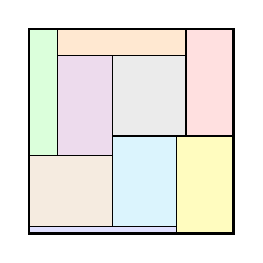
\begin{tikzpicture}[x=0.03023cm,y=0.03023cm]
\filldraw[fill=blue!12,draw=black,line width=0.4pt] (0,0) rectangle (62,3);
\filldraw[fill=orange!18,draw=black,line width=0.4pt] (12,75) rectangle (66,86);
\filldraw[fill=green!14,draw=black,line width=0.4pt] (0,33) rectangle (12,86);
\filldraw[fill=red!12,draw=black,line width=0.4pt] (66,41) rectangle (86,86);
\filldraw[fill=violet!14,draw=black,line width=0.4pt] (12,33) rectangle (35,75);
\filldraw[fill=yellow!25,draw=black,line width=0.4pt] (62,0) rectangle (86,41);
\filldraw[fill=cyan!14,draw=black,line width=0.4pt] (35,3) rectangle (62,41);
\filldraw[fill=brown!16,draw=black,line width=0.4pt] (0,3) rectangle (35,33);
\filldraw[fill=gray!16,draw=black,line width=0.4pt] (35,41) rectangle (66,75);
\draw[line width=0.9pt] (0,0) rectangle (86,86);
\end{tikzpicture}\\[2pt]{\footnotesize side 86, perimeter 130}
\end{minipage}\hfill
\begin{minipage}[b]{0.19\textwidth}\centering
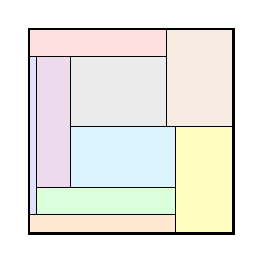
\begin{tikzpicture}[x=0.01615cm,y=0.01615cm]
\filldraw[fill=blue!12,draw=black,line width=0.4pt] (0,15) rectangle (6,139);
\filldraw[fill=orange!18,draw=black,line width=0.4pt] (0,0) rectangle (115,15);
\filldraw[fill=green!14,draw=black,line width=0.4pt] (6,15) rectangle (115,36);
\filldraw[fill=red!12,draw=black,line width=0.4pt] (0,139) rectangle (108,161);
\filldraw[fill=violet!14,draw=black,line width=0.4pt] (6,36) rectangle (33,139);
\filldraw[fill=yellow!25,draw=black,line width=0.4pt] (115,0) rectangle (161,84);
\filldraw[fill=cyan!14,draw=black,line width=0.4pt] (33,36) rectangle (115,84);
\filldraw[fill=brown!16,draw=black,line width=0.4pt] (108,84) rectangle (161,161);
\filldraw[fill=gray!16,draw=black,line width=0.4pt] (33,84) rectangle (108,139);
\draw[line width=0.9pt] (0,0) rectangle (161,161);
\end{tikzpicture}\\[2pt]{\footnotesize side 161, perimeter 260}
\end{minipage}\hfill
\begin{minipage}[b]{0.19\textwidth}\centering
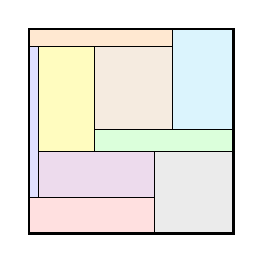
\begin{tikzpicture}[x=0.01576cm,y=0.01576cm]
\filldraw[fill=blue!12,draw=black,line width=0.4pt] (0,29) rectangle (8,151);
\filldraw[fill=orange!18,draw=black,line width=0.4pt] (0,151) rectangle (116,165);
\filldraw[fill=green!14,draw=black,line width=0.4pt] (53,66) rectangle (165,84);
\filldraw[fill=red!12,draw=black,line width=0.4pt] (0,0) rectangle (101,29);
\filldraw[fill=violet!14,draw=black,line width=0.4pt] (8,29) rectangle (101,66);
\filldraw[fill=yellow!25,draw=black,line width=0.4pt] (8,66) rectangle (53,151);
\filldraw[fill=cyan!14,draw=black,line width=0.4pt] (116,84) rectangle (165,165);
\filldraw[fill=brown!16,draw=black,line width=0.4pt] (53,84) rectangle (116,151);
\filldraw[fill=gray!16,draw=black,line width=0.4pt] (101,0) rectangle (165,66);
\draw[line width=0.9pt] (0,0) rectangle (165,165);
\end{tikzpicture}\\[2pt]{\footnotesize side 165, perimeter 260}
\end{minipage}

\caption{The five dissections of Theorem~\ref{thm:main}, each drawn at the same size.}
\label{fig:all5}
\end{figure}

The proof is computer-assisted but involves no floating point and no search heuristics. Section~\ref{sec:mechanism} shows why the equal-perimeter condition turns each combinatorial type of dissection into a square linear system, and Section~\ref{sec:computation} describes the enumeration and its checks.

\section{One equation per piece}\label{sec:mechanism}

Start with three pieces. Cut the unit square by a vertical line at distance $x$ from the left side, and cut the right-hand part by a horizontal line at height $y$, as in Figure~\ref{fig:mech}. Write $s$ for the common value of width plus height (half the perimeter). Each piece gives one equation:
\[
P_1:\ x+1=s,\qquad P_2:\ (1-x)+(1-y)=s,\qquad P_3:\ (1-x)+y=s .
\]
The left-hand side of each equation is the width plus the height of that piece, read off from the positions of the cuts. Three equations, three unknowns: subtracting the last two gives $y=\tfrac12$, and then $x=\tfrac14$, $s=\tfrac54$. So this arrangement of cuts has exactly one equal-perimeter version, and in it $P_2$ and $P_3$ are both $\tfrac34\times\tfrac12$. The arrangement fails, and nothing else could be tried for it, because the system left no freedom.

\begin{figure}[ht]
\centering
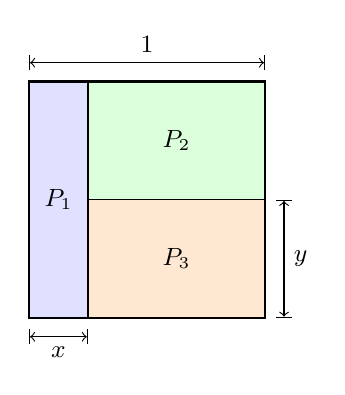
\begin{tikzpicture}[scale=3]
\filldraw[fill=blue!12] (0,0) rectangle (0.25,1);
\filldraw[fill=orange!18] (0.25,0) rectangle (1,0.5);
\filldraw[fill=green!14] (0.25,0.5) rectangle (1,1);
\draw[line width=0.9pt] (0,0) rectangle (1,1);
\node[font=\small] at (0.125,0.5) {$P_1$};
\node[font=\small] at (0.625,0.25) {$P_3$};
\node[font=\small] at (0.625,0.75) {$P_2$};
\draw[|<->|,thin] (0,-0.08) -- node[below,font=\small] {$x$} (0.25,-0.08);
\draw[|<->|,thin] (1.08,0) -- node[right,font=\small] {$y$} (1.08,0.5);
\draw[|<->|,thin] (0,1.08) -- node[above,font=\small] {$1$} (1,1.08);
\end{tikzpicture}

\caption{Three pieces. The positions $x$ and $y$ of the two cuts, together with the half-perimeter $s$, are the unknowns; each piece contributes one linear equation.}
\label{fig:mech}
\end{figure}

The same thing happens in general. In a dissection of a square into rectangles, a \emph{maximal segment} is a horizontal or vertical segment, contained in the union of the piece boundaries and not in the boundary of the square, that cannot be extended within that union. In Figure~\ref{fig:mech} there are two. The \emph{type} of a dissection records, for each piece, which maximal segment (or which side of the square) carries each of its four sides. Two dissections of the same type differ only in the positions of their maximal segments. A point inside the square where four pieces meet is a \emph{cross}.

\begin{lemma}\label{lem:count}
A dissection of a square into $n$ rectangles with $m$ maximal segments and $c$ crosses satisfies $n=m+c+1$.
\end{lemma}

\begin{proof}
Count the corners of the pieces, $4n$ in all, by where they sit. Each corner of the square is a corner of one piece. Each end of a maximal segment lies in the interior of another segment or of a side of the square, where it forms a T and is a corner of exactly two pieces; no point is an end of two maximal segments, since two collinear ends would join into one segment and two perpendicular ends would leave a piece with a reflex angle. A cross is a corner of four pieces. Every corner is of one of these three kinds, so $4n=4+2\cdot 2m+4c$.
\end{proof}

Without crosses, a type has $n-1$ maximal segments, each with one unknown position (its $x$-coordinate if vertical, its $y$-coordinate if horizontal). Fix the side of the square at $1$ and add the unknown half-perimeter $s$. Every piece gives the equation
\[
(\text{right} - \text{left}) + (\text{top} - \text{bottom}) = s ,
\]
where each of the four terms is the position of the segment or side that carries that side of the piece. This is $n$ linear equations in $n$ unknowns. When the system is nonsingular it has exactly one solution, so the type has at most one equal-perimeter realisation: the solution itself, and only if it gives every piece positive width and height. Call such a solution a \emph{candidate}.

A dissection with crosses is covered by the same systems. At each cross, regard the horizontal maximal segment through it as two segments that meet the vertical one from either side. The result is a type without crosses in which two horizontal segments happen to share a coordinate, and the given dissection is a realisation of that type. So every equal-perimeter dissection, with or without crosses, is the solution of the system of some cross-free type.

\section{The computation}\label{sec:computation}

To prove Theorem~\ref{thm:main} it therefore suffices to list every cross-free type with $n\le 9$ pieces, solve its system exactly over $\mathbb{Q}$, keep the candidates, and look among them for pieces that are pairwise non-congruent. Any candidate that survives must then be checked to be a genuine dissection. This was done twice, by programs that share no code.

\textbf{Program A} lists types directly. Cross-free types are known as mosaic floorplans, and their number for $n$ pieces is the Baxter number~\cite{yao}. The program builds them by repeatedly inserting a new piece at the top-left corner, in the manner of Nakano~\cite{nakano}, and removes duplicates by a canonical form. The counts agree with the Baxter numbers $1, 2, 6, 22, 92, 422, 2074, 10754, 58202$ for $n=1,\dots,9$.

\textbf{Program B} lists coordinate patterns instead. Given a cross-free dissection, nudge its maximal segments so that no two vertical ones and no two horizontal ones share a coordinate; a small enough move, with the ends of each segment sliding along the segments they meet, keeps the type. Replacing each coordinate by its rank then gives a tiling of a $(V+1)\times(H+1)$ grid of unit cells, where $V$ and $H$ are the numbers of vertical and horizontal segments, by $n=V+H+1$ rectangles, in which every interior grid line carries part of the boundary. Knuth calls these \emph{tight pavings}~\cite{knuth}. The program enumerates them by repeatedly filling the lowest, then leftmost, empty cell. A type can appear several times, once for each consistent ranking of its segments; that only repeats work. The counts agree with $1, 2, 6, 24, 118, 680, 4456, 32512, 260080$, the number of tight pavings with $n$ pieces summed over grid shapes~\cite{oeis298432}. The proof of Theorem~\ref{thm:main} rests on Program~A, whose completeness is that of Nakano's generation; Program~B is an independent check, so the nudging step, stated here without a detailed proof, is not needed for the theorem.

Both programs solve every system exactly, by Gauss--Jordan elimination over $\mathbb{Q}$ in Program~A and fraction-free Bareiss elimination in Program~B. Both find that \emph{every} system with $n\le 9$ is nonsingular. Both then compare the positive solutions as point sets, under the eight symmetries of the square, with the side scaled to $1$.

The number of inequivalent candidates found, with congruent pieces allowed, is
\[
1,\ 1,\ 2,\ 6,\ 16,\ 50,\ 177,\ 664,\ 2532 \qquad (n=1,\dots,9)
\]
in both programs. This agrees with the sequence computed earlier and independently by Beeksma and Riesebos~\cite{oeis100664}, which is a check on the whole pipeline: a missing type or a wrong equation would almost certainly change a count. Among these candidates, those with pairwise non-congruent pieces number $0$ for $2\le n\le 8$ and $5$ for $n=9$. A third script, which uses neither enumeration, checks directly from the integer coordinates in Table~\ref{tab:all5} that each of the five is a dissection of the square (pieces inside it, disjoint interiors, areas summing to the square), that all perimeters agree and that no two pieces are congruent. This completes the proof of Theorem~\ref{thm:main}.

The nonsingularity of every system is an observation, not a theorem. It is what makes each type contribute at most one dissection, and it was checked for each type rather than proved.

\begin{table}[ht]
\centering
\small
\begin{tabular}{@{}rrl@{}}
\toprule
side & perimeter & pieces, as $[x_1,x_2]\times[y_1,y_2]$ \\
\midrule
72 & 130 & \parbox[t]{0.74\textwidth}{\raggedright $[0,4]\times[11,72]$, $[0,55]\times[1,11]$, $[0,64]\times[0,1]$, $[4,22]\times[25,72]$, $[4,55]\times[11,25]$, $[22,55]\times[25,57]$, $[22,72]\times[57,72]$, $[55,64]\times[1,57]$, $[64,72]\times[0,57]$}\\[3pt]
84 & 130 & \parbox[t]{0.74\textwidth}{\raggedright $[0,10]\times[12,67]$, $[0,48]\times[67,84]$, $[0,53]\times[0,12]$, $[10,48]\times[40,67]$, $[10,53]\times[12,34]$, $[10,69]\times[34,40]$, $[48,69]\times[40,84]$, $[53,84]\times[0,34]$, $[69,84]\times[34,84]$}\\[3pt]
86 & 130 & \parbox[t]{0.74\textwidth}{\raggedright $[0,12]\times[33,86]$, $[0,35]\times[3,33]$, $[0,62]\times[0,3]$, $[12,35]\times[33,75]$, $[12,66]\times[75,86]$, $[35,62]\times[3,41]$, $[35,66]\times[41,75]$, $[62,86]\times[0,41]$, $[66,86]\times[41,86]$}\\[3pt]
161 & 260 & \parbox[t]{0.74\textwidth}{\raggedright $[0,6]\times[15,139]$, $[0,108]\times[139,161]$, $[0,115]\times[0,15]$, $[6,33]\times[36,139]$, $[6,115]\times[15,36]$, $[33,108]\times[84,139]$, $[33,115]\times[36,84]$, $[108,161]\times[84,161]$, $[115,161]\times[0,84]$}\\[3pt]
165 & 260 & \parbox[t]{0.74\textwidth}{\raggedright $[0,8]\times[29,151]$, $[0,101]\times[0,29]$, $[0,116]\times[151,165]$, $[8,53]\times[66,151]$, $[8,101]\times[29,66]$, $[53,116]\times[84,151]$, $[53,165]\times[66,84]$, $[101,165]\times[0,66]$, $[116,165]\times[84,165]$}\\[3pt]
\bottomrule
\end{tabular}

\caption{The five dissections of Theorem~\ref{thm:main}, in integer coordinates in lowest terms.}
\label{tab:all5}
\end{table}

\section{Remarks}

Among the nine-piece dissections, the smallest square with integer sides has side $72$; with more pieces a smaller one may exist. Nandakumar's guess that no square works~\cite[p.~5]{nandakumar} came with two others, about equal-perimeter rectangles with different areas tiling a rectangle that need not be square: that at least seven pieces are needed, and that the number of pieces may be bounded, since he knew of no example with more than ten. The method above does not settle these directly. For a rectangle the aspect ratio is one more unknown, so each type has a one-parameter family of solutions rather than a single point, and the question becomes whether some member of that family has all dimensions positive and all pieces different.

\textbf{Data and code.} The programs, their output and the checking script are in the folder \texttt{equal-perimeter-rectangles} of \url{https://github.com/jvvk/mathematics}.

\textbf{Acknowledgement.} The author used AI tools in developing this work and takes full responsibility for its content.

\begin{thebibliography}{9}

\bibitem{dalfo}
C.~Dalf\'o, M.~A.~Fiol, N.~L\'opez and A.~Mart\'inez-P\'erez, Decompositions of a rectangle into non-congruent rectangles of equal area, \emph{Discrete Math.} \textbf{344} (2021), no.~6, 112389, \href{https://doi.org/10.1016/j.disc.2021.112389}{doi:10.1016/j.disc.2021.112389}.

\bibitem{knuth}
D.~E.~Knuth, Problem 12005: Tight $m$-by-$n$ pavings, \emph{Amer. Math. Monthly} \textbf{124} (2017), no.~8, 754, \href{https://doi.org/10.4169/amer.math.monthly.124.8.754}{doi:10.4169/amer.math.monthly.124.8.754}; solution in \textbf{126} (2019), no.~7, 658--666, \href{https://doi.org/10.1080/00029890.2019.1621132}{doi:10.1080/00029890.2019.1621132}.

\bibitem{mo}
elbert k, Dividing a square into unique rectangles with the same perimeter, MathOverflow question 300255, 15 May 2018, \url{https://mathoverflow.net/q/300255}.

\bibitem{nakano}
S.~Nakano, Enumerating floorplans with $n$ rooms, in \emph{Algorithms and Computation (ISAAC 2001)}, Lecture Notes in Comput. Sci. \textbf{2223}, Springer, 2001, 107--115, \href{https://doi.org/10.1007/3-540-45678-3_10}{doi:10.1007/3-540-45678-3\_10}.

\bibitem{nandakumar}
R.~Nandakumar, A set of questions in combinatorial and metric geometry, arXiv:1307.3472v5 (2015), \url{https://arxiv.org/abs/1307.3472}.

\bibitem{oeis100664}
H.~Beeksma and H.~Riesebos, Number of inequivalent ways to dissect a square into $n$ rectangles of equal perimeter, sequence A100664 in \emph{The On-Line Encyclopedia of Integer Sequences}, \url{https://oeis.org/A100664}, accessed 8 October 2026.

\bibitem{oeis298432}
P.~Luschny, sequence A298432 in \emph{The On-Line Encyclopedia of Integer Sequences}, \url{https://oeis.org/A298432}, accessed 8 October 2026.

\bibitem{vanvera}
vanvera, Two dissection problems (xpost from geometry.puzzles), Usenet newsgroup \texttt{alt.math.recreational}, 19 November 2006, \url{https://groups.google.com/g/alt.math.recreational/c/I9ckSpjGHso}.

\bibitem{yao}
B.~Yao, H.~Chen, C.-K.~Cheng and R.~Graham, Floorplan representations: complexity and connections, \emph{ACM Trans. Des. Autom. Electron. Syst.} \textbf{8} (2003), no.~1, 55--80, \href{https://doi.org/10.1145/606603.606607}{doi:10.1145/606603.606607}.

\end{thebibliography}

\end{document}
